


\section{Linear calssification}
Some instance are linearly separable if it exists some hyper-plane that splits the space in two regions such that different classes are separated. Such hyper-plane is generated by a function $f$ which maps points in $\mathcal{R}^n$ to $C=\lbrace c_1,c_2,...,c_m\rbrace$
\[f: y(\bm{x})=\bm{w}^T\bm{x}+w_0\]


The problem with using multiple classes is shown in Figure \ref{fig:linear_problem}.


\begin{figure}[H]
    \centering
    \subfloat[One Versus One]{{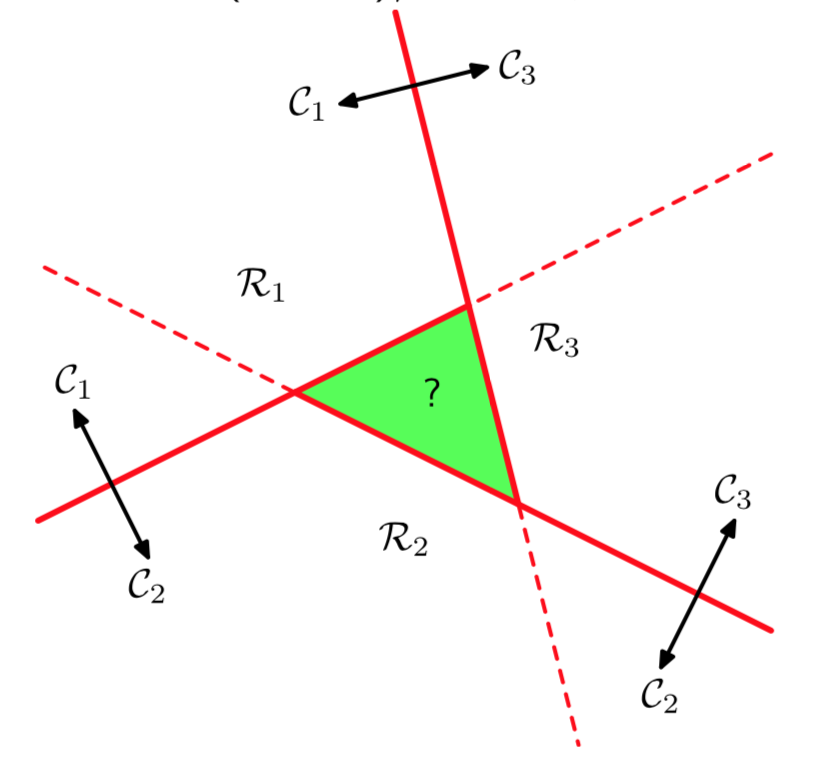
\includegraphics[width=5cm]{ovo_linear.png} }}%
    \qquad
    \subfloat[One Versus Rest]{{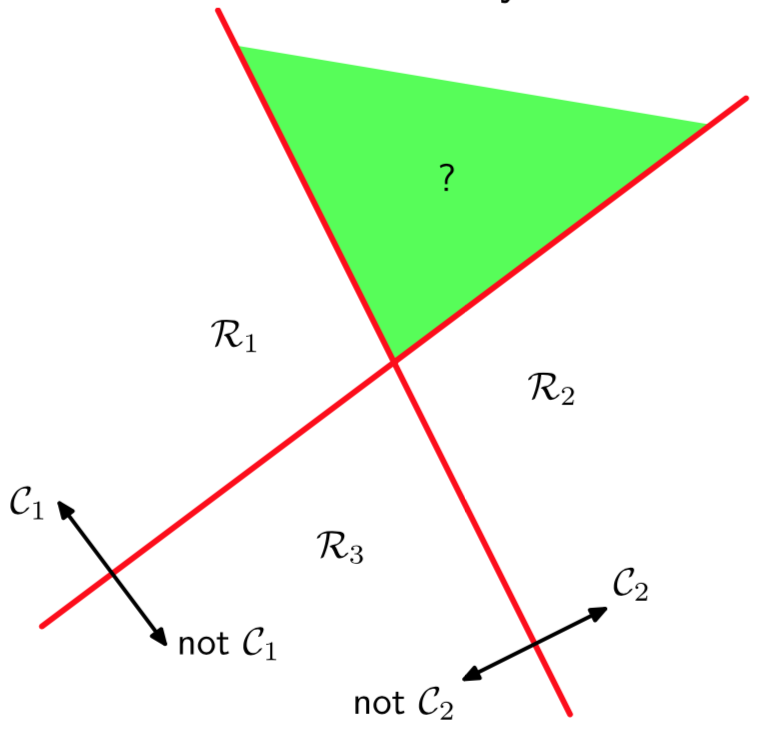
\includegraphics[width=5cm]{ovr_linear.png} }}%
    \caption{One Versus Rest }

\label{fig:linear_problem}%

\end{figure}


A solution is using a \textbf{K-Class Discriminant}:
\[f: y_k(\bm{x})=\bm{w}_k^T\bm{x}+w_{k0}\]
Where the decision boundary between two classes $C_j,C_k$, is given by:
\[(\bm{w_j}-\bm{w_k})^T\bm{x}+(w_{j0}-w{k0})\]
which can be written in a more compact notation having:
\begin{itemize}
\item $\cmp{w_k}=\binom{w_{k0}}{\bm{w_k}}$
\item $\cmp{x}=\binom{1}{\bm{x}}$
\item $\cmp{W}=(\bm{w_1},\bm{w_2},...\bm{w_k})$
\end{itemize}
We get:
\[\bm{y(x)}=\cmp{W}^T\cmp{x}\]
As shown in figure \ref{fig:k_discriminant}.

\begin{figure}[H]
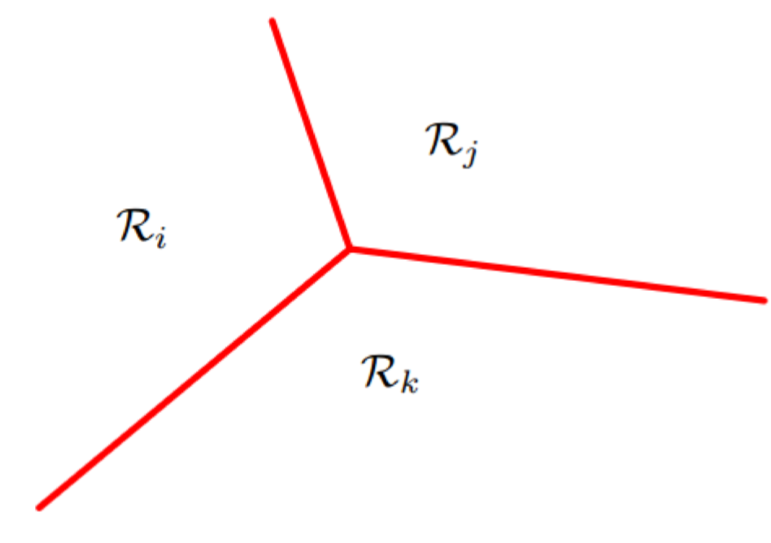
\includegraphics[scale=0.5]{k_discriminant.png}
\caption{K-class discriminant}
\label{fig:k_discriminant}
\end{figure}

Our goal is to determine a good $\cmp{W}$, there are various techniques we can use.

\subsection{Least Squares}
Given a dataset $D$ made of instances associated with a one hot vector encoder:
\[\forall x_i in D: iff x_i \in c_k \rightarrow t_i=(0,0,...,1,...0): t_i[k]=1\]
The Least Square aims to minimize the sum-of-square error function


\subsection{Fischer linear discriminant}
The main idea is to find projection to a line s.t. samples from different classes are well separated.\\
Suppose we have two classes and $n$ samples $x_1,...,x_n$ where $n_1$ samples are from class $1$ and $n_2$ are from $2$.\\
Considere a line which direction is given by a vector $v$, so that $v^tx_i$ is the projection of a point $x_i$ (2D) onto the line (1D).\\
We have that the mean of the points of classes $1$ is:
\[\mu_1=\frac{1}{n_1}\sum_{x_i \in C_1}^{n_1}x_i\]
Same thing for $\mu_2$. While the mean of the points \textbf{projected} onto the line is simply:
\[\tilde{\mu_1}=v^t\mu_1\]
So we can use $dist=|\tilde{\mu_1} -\tilde{\mu_2}|$ as a measure of separation, since the bigger the better, but look at Figure \ref{fig:fisher1}:

\begin{figure}[H]
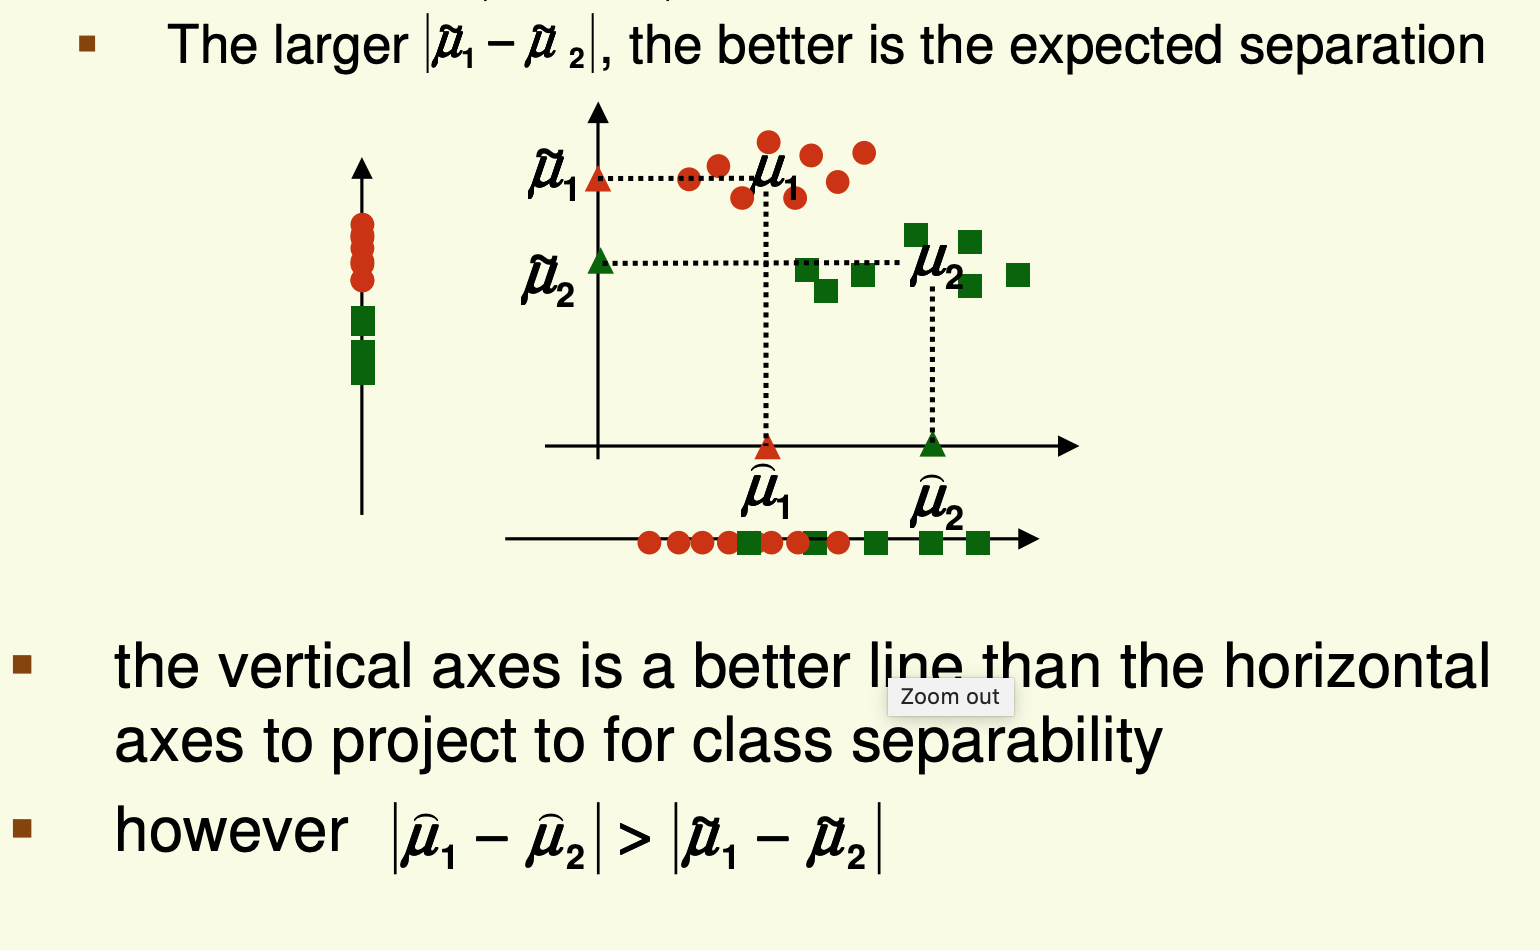
\includegraphics[scale=0.5]{fisher1.png}
\caption{Mean proble}
\label{fig:fisher1}
\end{figure}

The problem is that it does not consider the variance between classes, so we need to normalize $dist$ by something proportional to the variance.\\
Let's define the \textit{scatter} of some samples $z_1,...,z_n$ as :
\[s=\sum_{i=1}^n(z_i-\mu_z)^2\]
Which is:
\[s_1^2=\sum_{x_i \in C_1}(x_i-\tilde{\mu_1})^2\]
and the same for $s_2^2$
So we can now normalize the $dist$ by the scatter, getting the fisher linear discriminant:
\[J(v)=\frac{(\tilde{\mu_1}-\tilde{\mu_2})^2}{s_1^2-s_2^2}\]

\section{Perceptron}

\begin{figure}[H]
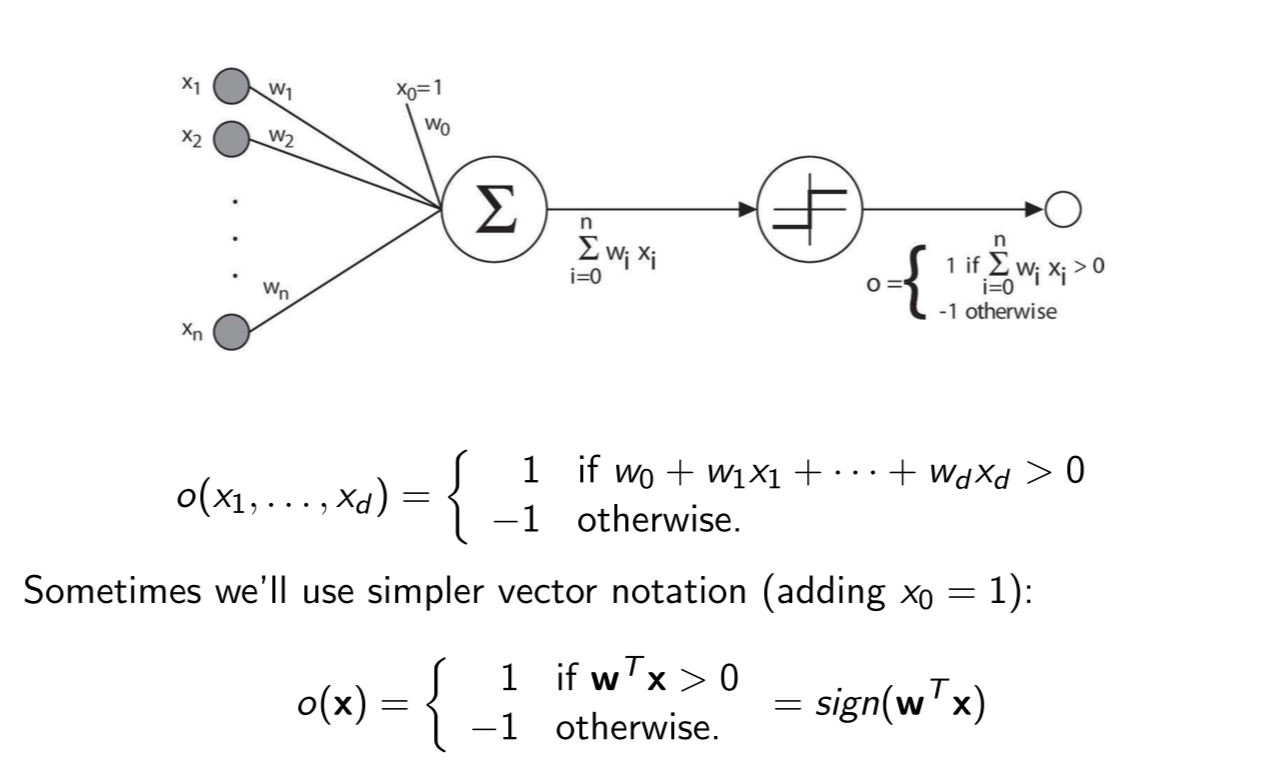
\includegraphics[scale=0.5]{perceptron.png}
\caption{Perceptron}
\label{fig:fisher1}
\end{figure}

The function to minimize is the square error, given the output $o$ and the true label $t$:
\[E(\bm{w})=\frac{1}{2}\sum_{n=1}^N(t_n-o_n)^2=\frac{1}{2}\sum_{n=1}^N(t_n -\bm{w}^Tx_n)^2\]
Since we need to minimize this error we want to move to the direction of the gradient, thus computing the derivative of:
\[\frac{\partialE(\bm{w}) }{\partial w_i}=\sum_{n=1}^N(t_n-\bm{w}^Tx_n)(-x_{i,n})\]
Where $-x_{i,n}$ is the value of i-th feature.\\
so we can update the weight $w_i$ by $w_{i+1}=w_i + \Delta w$, where:

\[\Delta w=-\eta \frac{\partial E(\bm{w}) }{\partial w_i}=\sum_{n=1}^N(t_n-sign(\bm{w}^Tx_n)))-x_{i,n} \]

\begin{figure}[H]
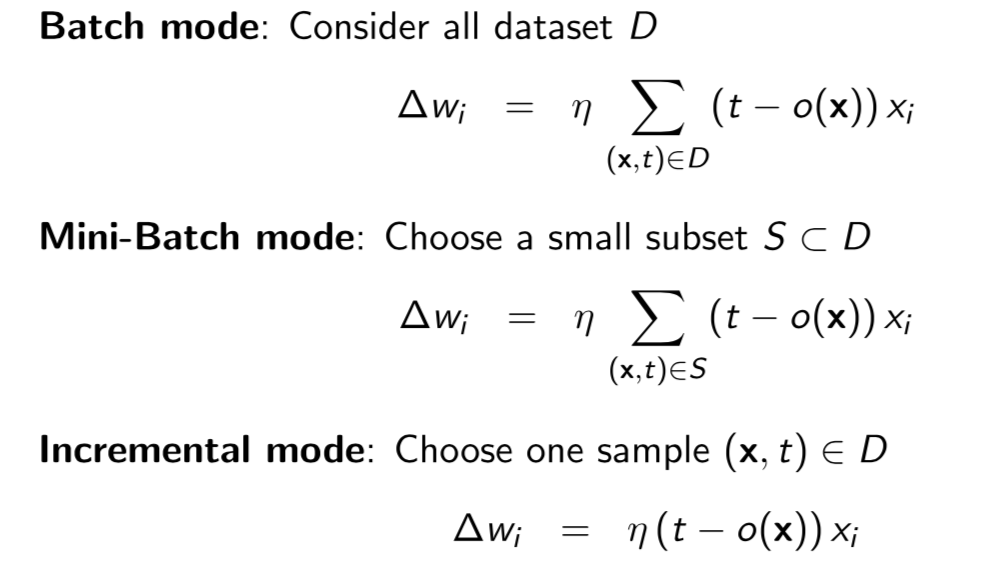
\includegraphics[scale=0.5]{perce_algh.png}
\caption{Perceptron Algotithm}
\end{figure}

\section{Support Vector Machine [SVM]}
SVMs are based on the idea of finding a hyperplane that best divides a dataset into two classes


\begin{figure}[H]
    \centering
    \subfloat{{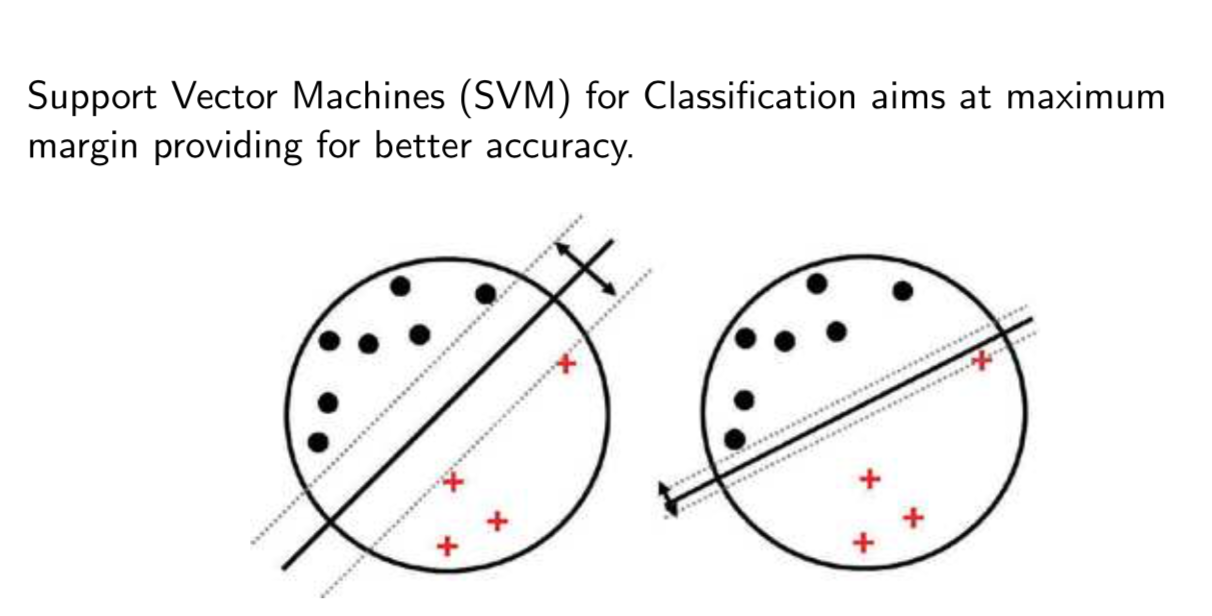
\includegraphics[width=5cm]{svm1.png} }}%
    \qquad
    \subfloat{{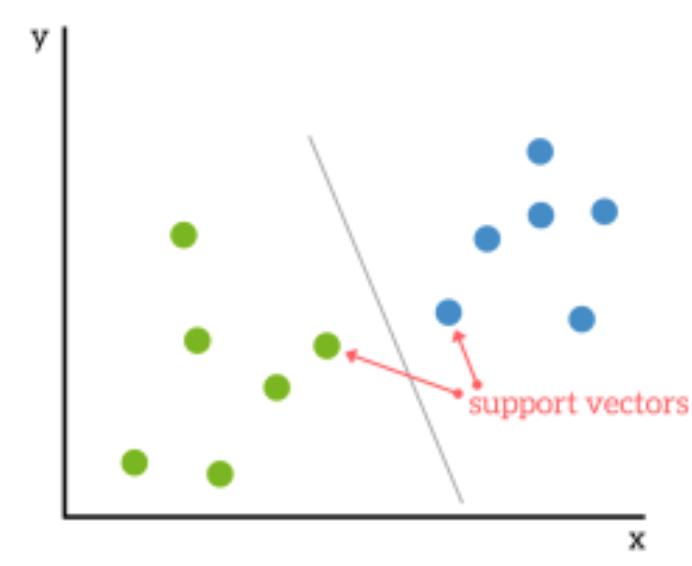
\includegraphics[width=5cm]{svm2.png} }}%

\label{fig:linear_problem}%
\end{figure}

Support vectors are the data points nearest to the hyperplane, the points of a data set that, if removed, would alter the position of the dividing hyperplane.\\
The distance between the hyperplane and the nearest data point from either set is known as the margin. The goal is to choose a hyperplane with the greatest possible margin between the hyperplane and any point within the training set, where the margin is estimated as:
\[\argmax_{\bm{w},w_0}\frac{1}{||\bm{w}||}\min_{n=1..N}[t_n(\bm{\hat{w}^Tx_n+\hat{w_0}})]\]
Where the
\begin{itemize}
\item $\hat{h}=\bm{\hat{w}^Tx_n+\hat{w_0}}$ is the hyperplane
\item $\frac{1}{||\bm{w}||}\min_{n=1..N}[t_n(\bm{\hat{w}^Tx_n+\hat{w_0}})]$ is the smallest distance between the hyperplane and $x$.

\end{itemize}
 

